\documentclass[]{book}
\usepackage{lmodern}
\usepackage{amssymb,amsmath}
\usepackage{ifxetex,ifluatex}
\usepackage{fixltx2e} % provides \textsubscript
\ifnum 0\ifxetex 1\fi\ifluatex 1\fi=0 % if pdftex
  \usepackage[T1]{fontenc}
  \usepackage[utf8]{inputenc}
\else % if luatex or xelatex
  \ifxetex
    \usepackage{mathspec}
  \else
    \usepackage{fontspec}
  \fi
  \defaultfontfeatures{Ligatures=TeX,Scale=MatchLowercase}
\fi
% use upquote if available, for straight quotes in verbatim environments
\IfFileExists{upquote.sty}{\usepackage{upquote}}{}
% use microtype if available
\IfFileExists{microtype.sty}{%
\usepackage{microtype}
\UseMicrotypeSet[protrusion]{basicmath} % disable protrusion for tt fonts
}{}
\usepackage[margin=1in]{geometry}
\usepackage{hyperref}
\hypersetup{unicode=true,
            pdftitle={Keeping track of notes, with the eventual hope of a book\ldots{}},
            pdfauthor={Mine Cetinkaya-Rundel},
            pdfborder={0 0 0},
            breaklinks=true}
\urlstyle{same}  % don't use monospace font for urls
\usepackage{natbib}
\bibliographystyle{apalike}
\usepackage{color}
\usepackage{fancyvrb}
\newcommand{\VerbBar}{|}
\newcommand{\VERB}{\Verb[commandchars=\\\{\}]}
\DefineVerbatimEnvironment{Highlighting}{Verbatim}{commandchars=\\\{\}}
% Add ',fontsize=\small' for more characters per line
\usepackage{framed}
\definecolor{shadecolor}{RGB}{248,248,248}
\newenvironment{Shaded}{\begin{snugshade}}{\end{snugshade}}
\newcommand{\KeywordTok}[1]{\textcolor[rgb]{0.13,0.29,0.53}{\textbf{#1}}}
\newcommand{\DataTypeTok}[1]{\textcolor[rgb]{0.13,0.29,0.53}{#1}}
\newcommand{\DecValTok}[1]{\textcolor[rgb]{0.00,0.00,0.81}{#1}}
\newcommand{\BaseNTok}[1]{\textcolor[rgb]{0.00,0.00,0.81}{#1}}
\newcommand{\FloatTok}[1]{\textcolor[rgb]{0.00,0.00,0.81}{#1}}
\newcommand{\ConstantTok}[1]{\textcolor[rgb]{0.00,0.00,0.00}{#1}}
\newcommand{\CharTok}[1]{\textcolor[rgb]{0.31,0.60,0.02}{#1}}
\newcommand{\SpecialCharTok}[1]{\textcolor[rgb]{0.00,0.00,0.00}{#1}}
\newcommand{\StringTok}[1]{\textcolor[rgb]{0.31,0.60,0.02}{#1}}
\newcommand{\VerbatimStringTok}[1]{\textcolor[rgb]{0.31,0.60,0.02}{#1}}
\newcommand{\SpecialStringTok}[1]{\textcolor[rgb]{0.31,0.60,0.02}{#1}}
\newcommand{\ImportTok}[1]{#1}
\newcommand{\CommentTok}[1]{\textcolor[rgb]{0.56,0.35,0.01}{\textit{#1}}}
\newcommand{\DocumentationTok}[1]{\textcolor[rgb]{0.56,0.35,0.01}{\textbf{\textit{#1}}}}
\newcommand{\AnnotationTok}[1]{\textcolor[rgb]{0.56,0.35,0.01}{\textbf{\textit{#1}}}}
\newcommand{\CommentVarTok}[1]{\textcolor[rgb]{0.56,0.35,0.01}{\textbf{\textit{#1}}}}
\newcommand{\OtherTok}[1]{\textcolor[rgb]{0.56,0.35,0.01}{#1}}
\newcommand{\FunctionTok}[1]{\textcolor[rgb]{0.00,0.00,0.00}{#1}}
\newcommand{\VariableTok}[1]{\textcolor[rgb]{0.00,0.00,0.00}{#1}}
\newcommand{\ControlFlowTok}[1]{\textcolor[rgb]{0.13,0.29,0.53}{\textbf{#1}}}
\newcommand{\OperatorTok}[1]{\textcolor[rgb]{0.81,0.36,0.00}{\textbf{#1}}}
\newcommand{\BuiltInTok}[1]{#1}
\newcommand{\ExtensionTok}[1]{#1}
\newcommand{\PreprocessorTok}[1]{\textcolor[rgb]{0.56,0.35,0.01}{\textit{#1}}}
\newcommand{\AttributeTok}[1]{\textcolor[rgb]{0.77,0.63,0.00}{#1}}
\newcommand{\RegionMarkerTok}[1]{#1}
\newcommand{\InformationTok}[1]{\textcolor[rgb]{0.56,0.35,0.01}{\textbf{\textit{#1}}}}
\newcommand{\WarningTok}[1]{\textcolor[rgb]{0.56,0.35,0.01}{\textbf{\textit{#1}}}}
\newcommand{\AlertTok}[1]{\textcolor[rgb]{0.94,0.16,0.16}{#1}}
\newcommand{\ErrorTok}[1]{\textcolor[rgb]{0.64,0.00,0.00}{\textbf{#1}}}
\newcommand{\NormalTok}[1]{#1}
\usepackage{longtable,booktabs}
\usepackage{graphicx,grffile}
\makeatletter
\def\maxwidth{\ifdim\Gin@nat@width>\linewidth\linewidth\else\Gin@nat@width\fi}
\def\maxheight{\ifdim\Gin@nat@height>\textheight\textheight\else\Gin@nat@height\fi}
\makeatother
% Scale images if necessary, so that they will not overflow the page
% margins by default, and it is still possible to overwrite the defaults
% using explicit options in \includegraphics[width, height, ...]{}
\setkeys{Gin}{width=\maxwidth,height=\maxheight,keepaspectratio}
\IfFileExists{parskip.sty}{%
\usepackage{parskip}
}{% else
\setlength{\parindent}{0pt}
\setlength{\parskip}{6pt plus 2pt minus 1pt}
}
\setlength{\emergencystretch}{3em}  % prevent overfull lines
\providecommand{\tightlist}{%
  \setlength{\itemsep}{0pt}\setlength{\parskip}{0pt}}
\setcounter{secnumdepth}{5}
% Redefines (sub)paragraphs to behave more like sections
\ifx\paragraph\undefined\else
\let\oldparagraph\paragraph
\renewcommand{\paragraph}[1]{\oldparagraph{#1}\mbox{}}
\fi
\ifx\subparagraph\undefined\else
\let\oldsubparagraph\subparagraph
\renewcommand{\subparagraph}[1]{\oldsubparagraph{#1}\mbox{}}
\fi

%%% Use protect on footnotes to avoid problems with footnotes in titles
\let\rmarkdownfootnote\footnote%
\def\footnote{\protect\rmarkdownfootnote}

%%% Change title format to be more compact
\usepackage{titling}

% Create subtitle command for use in maketitle
\newcommand{\subtitle}[1]{
  \posttitle{
    \begin{center}\large#1\end{center}
    }
}

\setlength{\droptitle}{-2em}
  \title{Keeping track of notes, with the eventual hope of a book\ldots{}}
  \pretitle{\vspace{\droptitle}\centering\huge}
  \posttitle{\par}
  \author{Mine Cetinkaya-Rundel}
  \preauthor{\centering\large\emph}
  \postauthor{\par}
  \predate{\centering\large\emph}
  \postdate{\par}
  \date{2018-02-02}

\usepackage{booktabs}
\usepackage{amsthm}
\makeatletter
\def\thm@space@setup{%
  \thm@preskip=8pt plus 2pt minus 4pt
  \thm@postskip=\thm@preskip
}
\makeatother

\usepackage{amsthm}
\newtheorem{theorem}{Theorem}[chapter]
\newtheorem{lemma}{Lemma}[chapter]
\theoremstyle{definition}
\newtheorem{definition}{Definition}[chapter]
\newtheorem{corollary}{Corollary}[chapter]
\newtheorem{proposition}{Proposition}[chapter]
\theoremstyle{definition}
\newtheorem{example}{Example}[chapter]
\theoremstyle{definition}
\newtheorem{exercise}{Exercise}[chapter]
\theoremstyle{remark}
\newtheorem*{remark}{Remark}
\newtheorem*{solution}{Solution}
\begin{document}
\maketitle

{
\setcounter{tocdepth}{1}
\tableofcontents
}
\begin{Shaded}
\begin{Highlighting}[]
\KeywordTok{library}\NormalTok{(tidyverse)}
\end{Highlighting}
\end{Shaded}

\chapter{Lab 3 - Visualizing spatial
data}\label{lab-3---visualizing-spatial-data}

\section{Introduction}\label{introduction}

Have you ever taken a road trip in the US and thought to yourself ``I
wonder what La Quinta means''. Well, the late comedian
\href{https://en.wikipedia.org/wiki/Mitch_Hedberg}{Mitch Hedberg} thinks
it's Spanish for \emph{next to Denny's}.

If you're not familiar with these two establishments,
\href{https://www.dennys.com/}{Denny's} is a casual diner chain that is
open 24 hours and \href{http://www.lq.com/}{La Quinta Inn and Suites} is
a hotel chain.

\begin{figure}
\centering
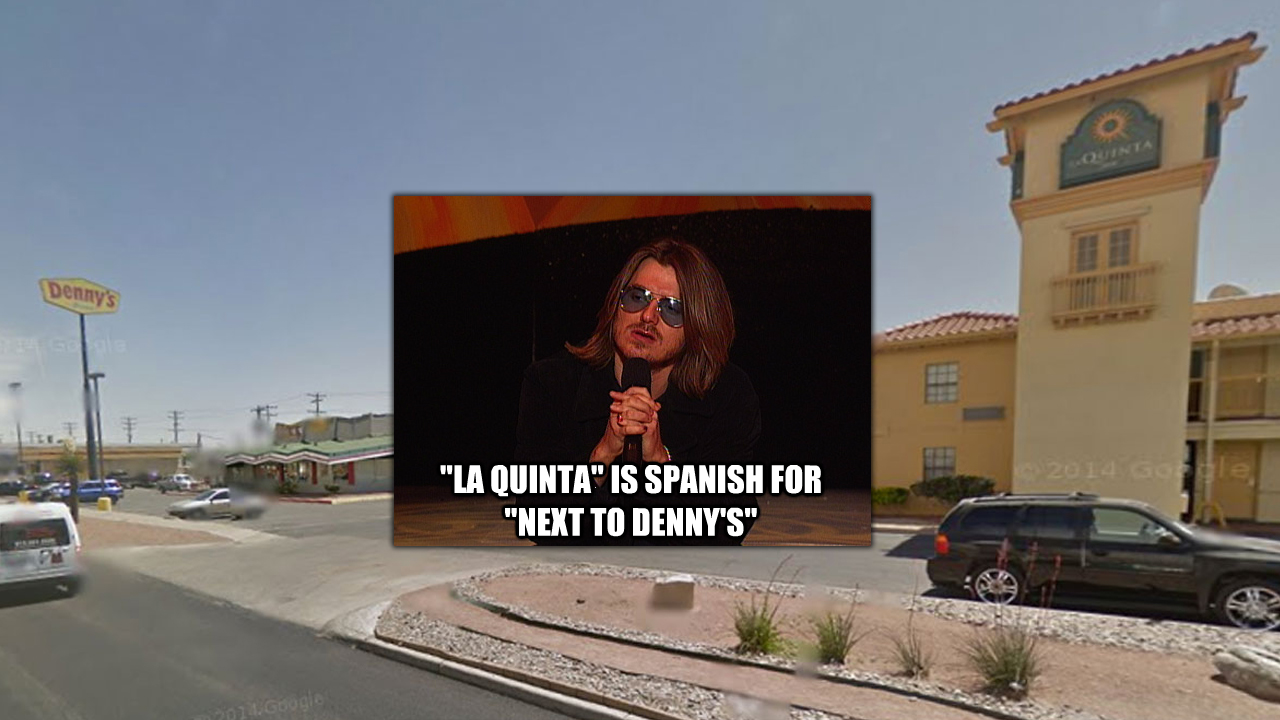
\includegraphics{img/03-viz-sp-data/mitch-hedgeberg-lqd.jpg}
\caption{LA Quinta is Spanish for next to Denny's}
\end{figure}

These two establishments tend to be clustered together, or at least this
observation is a joke made famous by Mitch Hedberg. In this lab we
explore the validity of this joke and along the way learn some more data
wrangling and tips for visualizing spatial data.

The inspiration for this lab comes from a blog post by John Reiser on
his \emph{new jersey geographer} blog. You can read that analysis
\href{http://njgeo.org/2014/01/30/mitch-hedberg-and-gis/}{here}.
Reiser's blog post focuses on scraping data from Denny's and La Quinta
Inn and Suites websites using Python. In this lab we focus on
visualization and analysis of these data. However note that the data
scraping was also done in R, and we we will discuss web scraping using R
later in the course. But for now we focus on the data that has already
been scraped and tidied for you.

\chapter{Getting started}\label{getting-started}

\begin{itemize}
\item
  Go to the course organization on GitHub:
  \url{https://github.com/Sta199-S18}.
\item
  Find the repo starting with \texttt{lab-03} and that has your team
  name at the end (this should be the only \texttt{lab-03} repo
  available to you).
\item
  In the repo, click on the green \textbf{Clone or download} button,
  select \textbf{Use HTTPS} (this might already be selected by default,
  and if it is, you'll see the text \textbf{Clone with HTTPS} as in the
  image below). Click on the clipboard icon to copy the repo URL.
\item
  Go to RStudio Cloud and into the course workspace. Create a
  \textbf{New Project from Git Repo}. You will need to click on the down
  arrow next to the \textbf{New Project} button to see this option.
\item
  Copy and paste the URL of your assignment repo into the dialog box:
\item
  Hit OK, and you're good to go!
\end{itemize}

\chapter{Packages}\label{packages}

In this lab we will work with the \texttt{tidyverse} package. So we need
to install and load it:

\begin{Shaded}
\begin{Highlighting}[]
\KeywordTok{install.packages}\NormalTok{(}\StringTok{"tidyverse"}\NormalTok{)}
\KeywordTok{library}\NormalTok{(tidyverse) }
\end{Highlighting}
\end{Shaded}

Note that this package is also loaded in your R Markdown document.

\chapter{Housekeeping}\label{housekeeping}

\section{Git configuration}\label{git-configuration}

Your email address is the address tied to your GitHub account and your
name should be first and last name.

\begin{itemize}
\tightlist
\item
  Go to the \emph{Terminal} pane
\item
  Type the following two lines of code, replacing the information in the
  quotation marks with your info.
\end{itemize}

\begin{Shaded}
\begin{Highlighting}[]
\FunctionTok{git}\NormalTok{ config --global user.email }\StringTok{"your email"}
\FunctionTok{git}\NormalTok{ config --global user.name }\StringTok{"your name"}
\end{Highlighting}
\end{Shaded}

To confirm that the changes have been implemented, run the following:

\begin{Shaded}
\begin{Highlighting}[]
\FunctionTok{git}\NormalTok{ config --global user.email}
\FunctionTok{git}\NormalTok{ config --global user.name}
\end{Highlighting}
\end{Shaded}

\section{Project name:}\label{project-name}

Currently your project is called \emph{Untitled Project}. Update the
name of your project to be ``Lab 03 - Visualizing spatial data''.

\chapter{Warm up}\label{warm-up}

\textbf{Pick one team member to complete the steps in this section while
the others contribute to the discussion but do not actually touch the
files on their computer.}

Before we introduce the data, let's warm up with some simple exercises.

\section{YAML:}\label{yaml}

Open the R Markdown (Rmd) file in your project, change the author name
to your \textbf{team} name, and knit the document.

\section{Commiting and pushing
changes:}\label{commiting-and-pushing-changes}

\begin{itemize}
\tightlist
\item
  Go to the \textbf{Git} pane in your RStudio.
\item
  View the \textbf{Diff} and confirm that you are happy with the
  changes.
\item
  Add a commit message like ``Update team name'' in the \textbf{Commit
  message} box and hit \textbf{Commit}.
\item
  Click on \textbf{Push}. This will prompt a dialogue box where you
  first need to enter your user name, and then your password.
\end{itemize}

\section{Pulling changes:}\label{pulling-changes}

Now, the remaining team members who have not been concurrently making
these changes on their projects should click on the \textbf{Pull} button
in their Git pane and observe that the changes are now reflected on
their projects as well.

\chapter{The data}\label{the-data}

The data consist of two csv (comma separated values) files: one for
Denny's locations and the other for La Quinta.

\begin{Shaded}
\begin{Highlighting}[]
\NormalTok{dn <-}\StringTok{ }\KeywordTok{read_csv}\NormalTok{(}\StringTok{"data/dennys.csv"}\NormalTok{)}
\end{Highlighting}
\end{Shaded}

\begin{verbatim}
## Parsed with column specification:
## cols(
##   address = col_character(),
##   city = col_character(),
##   state = col_character(),
##   zip = col_character(),
##   longitude = col_double(),
##   latitude = col_double()
## )
\end{verbatim}

\begin{Shaded}
\begin{Highlighting}[]
\NormalTok{lq <-}\StringTok{ }\KeywordTok{read_csv}\NormalTok{(}\StringTok{"data/laquinta.csv"}\NormalTok{)}
\end{Highlighting}
\end{Shaded}

\begin{verbatim}
## Parsed with column specification:
## cols(
##   address = col_character(),
##   city = col_character(),
##   state = col_character(),
##   zip = col_character(),
##   longitude = col_double(),
##   latitude = col_double()
## )
\end{verbatim}

Note that these data were scraped from
\href{https://locations.dennys.com/}{here} and
\href{https://www.lq.com/en/findandbook/hotel-listings.html}{here},
respectively.

To help with our analysis we will also use a dataset on US states:

\begin{Shaded}
\begin{Highlighting}[]
\NormalTok{states <-}\StringTok{ }\KeywordTok{read_csv}\NormalTok{(}\StringTok{"data/states.csv"}\NormalTok{)}
\end{Highlighting}
\end{Shaded}

\begin{verbatim}
## Parsed with column specification:
## cols(
##   name = col_character(),
##   abbreviation = col_character(),
##   area = col_double()
## )
\end{verbatim}

Each observation in this dataset represents a state, including DC. Along
with the name of the state we have the two-letter abbreviation and we
have the geographic area of the state (in square miles).

\chapter{Exercises}\label{exercises}

\textbf{Exercise 1:} What are the dimensions of the Denny's dataset?
(Hint: Use inline R code and functions like \texttt{nrow} and
\texttt{ncol} to compose your answer.) What does each row in the dataset
represent? What are the variables?

\textbf{Exercise 2:} What are the dimensions of the La Quinta's dataset?
What does each row in the dataset represent? What are the variables?

We would like to limit our analysis to Denny's and La Quinta locations
in the United States.

\textbf{Exercise 3:} Take a look at the websites that the data come from
(linked above). Are there any La Quinta's locations outside of the US?
If so, which countries? What about Denny's?

\textbf{Exercise 4:} Now take a look at the data. What would be some
ways of determining whether or not either establishment has any
locations outside the US using just the data (and not the websites).
Don't worry about whether you know how to implement this, just
brainstorm some ideas. Write down at least one as your answer, but
you're welcomed to write down a few options too.

We will determine whether or not the establishment has a location
outside the US using the \texttt{state} variable in the \texttt{dn} and
\texttt{lq} datasets. We know exactly which states are in the US, and we
have this information in the \texttt{states} dataframe we loaded.

\textbf{Exercise 5:} Find the Denny's locations that are outside the US,
if any. To do so, filter the Denny's locations for observations where
\texttt{state} is not in \texttt{states\$abbreviation}. The code for
this is given below. Note that the \texttt{\%in\%} operator matches the
states listed in the \texttt{state} variable to those listed in
\texttt{states\$abbreviation}. The \texttt{!} operator means
\textbf{not}. Are there any Denny's locations outside the US?

``Filter for \texttt{state}s that are not in
\texttt{states\$abbreviation}.''

\begin{Shaded}
\begin{Highlighting}[]
\NormalTok{dn }\OperatorTok
\StringTok{  }\KeywordTok{filter}\NormalTok{(}\OperatorTok{!}\NormalTok{(state }\OperatorTok\StringTok{ }\NormalTok{states}\OperatorTok{$}\NormalTok{abbreviation))}
\end{Highlighting}
\end{Shaded}

\begin{verbatim}
## # A tibble: 0 x 6
## # ... with 6 variables: address <chr>, city <chr>, state <chr>, zip <chr>,
## #   longitude <dbl>, latitude <dbl>
\end{verbatim}

\textbf{Exercise 6:} Add a country variable to the Denny's dataset and
set all observations equal to \texttt{"United\ States"}. Remember, you
can use the \texttt{mutate} function for adding a variable.

We don't need to tell R how many times to repeat the character string
``United States'' to fill in the data for all observations, R takes care
of that automatically.

\begin{Shaded}
\begin{Highlighting}[]
\NormalTok{dn }\OperatorTok
\StringTok{  }\KeywordTok{mutate}\NormalTok{(}\DataTypeTok{country =} \StringTok{"United States"}\NormalTok{)}
\end{Highlighting}
\end{Shaded}

\begin{verbatim}
## # A tibble: 1,643 x 7
##    address            city        state zip   longitude latitude country  
##    <chr>              <chr>       <chr> <chr>     <dbl>    <dbl> <chr>    
##  1 2900 Denali        Anchorage   AK    99503    -150       61.2 United S~
##  2 3850 Debarr Road   Anchorage   AK    99508    -150       61.2 United S~
##  3 1929 Airport Way   Fairbanks   AK    99701    -148       64.8 United S~
##  4 230 Connector Dr   Auburn      AL    36849    - 85.5     32.6 United S~
##  5 224 Daniel Payne ~ Birmingham  AL    35207    - 86.8     33.6 United S~
##  6 900 16th St S, Co~ Birmingham  AL    35294    - 86.8     33.5 United S~
##  7 5931 Alabama High~ Cullman     AL    35056    - 86.9     34.2 United S~
##  8 2190 Ross Clark C~ Dothan      AL    36301    - 85.4     31.2 United S~
##  9 900 Tyson Rd       Hope Hull ~ AL    36043    - 86.4     32.2 United S~
## 10 4874 University D~ Huntsville  AL    35816    - 86.7     34.7 United S~
## # ... with 1,633 more rows
\end{verbatim}

Make sure to save the result of this as \texttt{dn} again so that the
stored data frame contains the new variable going forward.

\textbf{Exercise 7:} Find the La Quinta locations that are outside the
US, and figure out which country they are in. This might require some
googling. Take notes, you will need to use this information in the next
exercise.

\textbf{Exercise 8:} Add a country variable to the La Quinta dataset.
Use the \texttt{case\_when} function to populate this variable. You'll
need to refer to your notes from Exercise 7 about which country the
non-US locations are in. Here is some starter code to get you going:

\begin{Shaded}
\begin{Highlighting}[]
\NormalTok{lq }\OperatorTok
\StringTok{  }\KeywordTok{mutate}\NormalTok{(}\DataTypeTok{country =} \KeywordTok{case_when}\NormalTok{(}
\NormalTok{    state }\OperatorTok\StringTok{ }\NormalTok{state.abb     }\OperatorTok{~}\StringTok{ "United States"}\NormalTok{,}
\NormalTok{    state }\OperatorTok\StringTok{ }\KeywordTok{c}\NormalTok{(}\StringTok{"ON"}\NormalTok{, }\StringTok{"BC"}\NormalTok{) }\OperatorTok{~}\StringTok{ "Canada"}\NormalTok{,}
\NormalTok{    state }\OperatorTok{==}\StringTok{ "ANT"}           \OperatorTok{~}\StringTok{ "Colombia"}\NormalTok{,}
\NormalTok{    ...                      }\CommentTok{# fill in the rest}
\NormalTok{  ))}
\end{Highlighting}
\end{Shaded}

Going forward we will work with the data from the United States only.
All Denny's locations are in the United States, so we don't need to
worry about them. However we do need to filter the La Quinta dataset for
locations in United States.

\begin{Shaded}
\begin{Highlighting}[]
\NormalTok{lq <-}\StringTok{ }\NormalTok{lq }\OperatorTok
\StringTok{  }\KeywordTok{filter}\NormalTok{(country }\OperatorTok{==}\StringTok{ "United States"}\NormalTok{)}
\end{Highlighting}
\end{Shaded}

\textbf{Exercise 9:} Which states have the most and fewest Denny's
locations? What about La Quinta? Is this surprising? Why or why not?

Next, let's calculate which states have the most Denny's locations
\emph{per thousand square miles}. This requires joinining information
from the frequency tables you created in Exercise 8 with information
from the \texttt{states} data frame.

First, we count how many observations are in each state, which will give
us a data frame with two variables: \texttt{state} and \texttt{n}. Then,
we join this data frame with the \texttt{states} data frame. However
note that the variables in the \texttt{states} data frame that has the
two-letter abbreviations is called \texttt{abbreviation}. So when we're
joining the two data frames we specify that the \texttt{state} variable
from the Denny's data should be matched \texttt{by} the
\texttt{abbreviation} variable from the \texttt{states} data:

\begin{Shaded}
\begin{Highlighting}[]
\NormalTok{dn }\OperatorTok
\StringTok{  }\KeywordTok{count}\NormalTok{(state) }\OperatorTok
\StringTok{  }\KeywordTok{inner_join}\NormalTok{(states, }\DataTypeTok{by =} \KeywordTok{c}\NormalTok{(}\StringTok{"state"}\NormalTok{ =}\StringTok{ "abbreviation"}\NormalTok{))}
\end{Highlighting}
\end{Shaded}

Before you move on the the next question, run the code above and take a
look at the output. In the next exercise you will need to build on this
pipe.

\textbf{Exercise 10:} Which states have the most Denny's locations per
thousand square miles? What about La Quinta?

Next, we put the two datasets together into a single data frame. However
before we do so, we need to add an identifier variable. We'll call this
\texttt{establishment} and set the value to
\texttt{"Denny\textquotesingle{}s"} and \texttt{"La\ Quinta"} for the
\texttt{dn} and \texttt{lq} data frames, respectively.

\begin{Shaded}
\begin{Highlighting}[]
\NormalTok{dn <-}\StringTok{ }\NormalTok{dn }\OperatorTok
\StringTok{  }\KeywordTok{mutate}\NormalTok{(}\DataTypeTok{establishment =} \StringTok{"Denny's"}\NormalTok{)}
\NormalTok{lq <-}\StringTok{ }\NormalTok{lq }\OperatorTok
\StringTok{  }\KeywordTok{mutate}\NormalTok{(}\DataTypeTok{establishment =} \StringTok{"La Quinta"}\NormalTok{)}
\end{Highlighting}
\end{Shaded}

Since the two data frames have the same columns, we can easily bind them
with the \texttt{bind\_rows} function:

\begin{Shaded}
\begin{Highlighting}[]
\NormalTok{dn_lq <-}\StringTok{ }\KeywordTok{bind_rows}\NormalTok{(dn, lq)}
\end{Highlighting}
\end{Shaded}

We can plot the locations of the two establishments using a scatter
plot, and color the points by the establishment type. Note that the
latitude is plotted on the x-axis and the longitude on the y-axis.

\begin{Shaded}
\begin{Highlighting}[]
\KeywordTok{ggplot}\NormalTok{(dn_lq, }\DataTypeTok{mapping =} \KeywordTok{aes}\NormalTok{(}\DataTypeTok{x =}\NormalTok{ longitude, }\DataTypeTok{y =}\NormalTok{ latitude, }\DataTypeTok{color =}\NormalTok{ establishment)) }\OperatorTok{+}
\StringTok{  }\KeywordTok{geom_point}\NormalTok{()}
\end{Highlighting}
\end{Shaded}

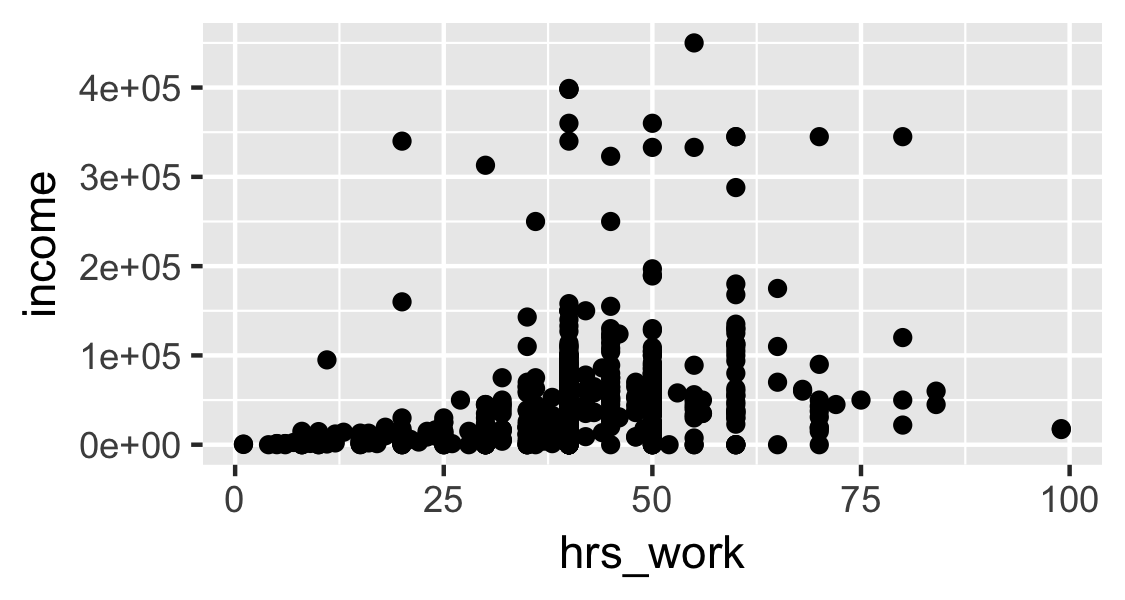
\includegraphics{bookdown-demo_files/figure-latex/unnamed-chunk-15-1.pdf}

See \href{http://ggplot2.tidyverse.org/reference/labs.html}{here} for
help with the syntax for customizing your plots. You can also choose
different themes to change the overall look of your plots, see
\href{http://ggplot2.tidyverse.org/reference/ggtheme.html}{here} for
help with these.

The following two questions ask you to create visualizations. These
should follow best practices you learned in class, such as informative
titles, axis labels, etc.

\textbf{Exercise 11:} Filter the data for observations in North Carolina
only, and recreate the plot. You should also adjust the transparency of
the points, by setting the \texttt{alpha} level, so that it's easier to
see the overplotted ones. Visually, does Mitch Hedberg's joke appear to
hold here?

\textbf{Exercise 12:} Now filter the data for observations in Texas
only, and recreate the plot, with an appropriate \texttt{alpha} level.
Visually, does Mitch Hedberg's joke appear to hold here?

That's it for now! In the next lab we will take a more quantitative
approach to answering these questions.

\bibliography{book.bib,packages.bib}


\end{document}
